% Options for packages loaded elsewhere
\PassOptionsToPackage{unicode}{hyperref}
\PassOptionsToPackage{hyphens}{url}
%
\documentclass[
]{book}
\usepackage{amsmath,amssymb}
\usepackage{lmodern}
\usepackage{iftex}
\ifPDFTeX
  \usepackage[T1]{fontenc}
  \usepackage[utf8]{inputenc}
  \usepackage{textcomp} % provide euro and other symbols
\else % if luatex or xetex
  \usepackage{unicode-math}
  \defaultfontfeatures{Scale=MatchLowercase}
  \defaultfontfeatures[\rmfamily]{Ligatures=TeX,Scale=1}
\fi
% Use upquote if available, for straight quotes in verbatim environments
\IfFileExists{upquote.sty}{\usepackage{upquote}}{}
\IfFileExists{microtype.sty}{% use microtype if available
  \usepackage[]{microtype}
  \UseMicrotypeSet[protrusion]{basicmath} % disable protrusion for tt fonts
}{}
\makeatletter
\@ifundefined{KOMAClassName}{% if non-KOMA class
  \IfFileExists{parskip.sty}{%
    \usepackage{parskip}
  }{% else
    \setlength{\parindent}{0pt}
    \setlength{\parskip}{6pt plus 2pt minus 1pt}}
}{% if KOMA class
  \KOMAoptions{parskip=half}}
\makeatother
\usepackage{xcolor}
\IfFileExists{xurl.sty}{\usepackage{xurl}}{} % add URL line breaks if available
\IfFileExists{bookmark.sty}{\usepackage{bookmark}}{\usepackage{hyperref}}
\hypersetup{
  pdftitle={A Minimal Book Example},
  pdfauthor={John Doe},
  hidelinks,
  pdfcreator={LaTeX via pandoc}}
\urlstyle{same} % disable monospaced font for URLs
\usepackage{color}
\usepackage{fancyvrb}
\newcommand{\VerbBar}{|}
\newcommand{\VERB}{\Verb[commandchars=\\\{\}]}
\DefineVerbatimEnvironment{Highlighting}{Verbatim}{commandchars=\\\{\}}
% Add ',fontsize=\small' for more characters per line
\usepackage{framed}
\definecolor{shadecolor}{RGB}{248,248,248}
\newenvironment{Shaded}{\begin{snugshade}}{\end{snugshade}}
\newcommand{\AlertTok}[1]{\textcolor[rgb]{0.94,0.16,0.16}{#1}}
\newcommand{\AnnotationTok}[1]{\textcolor[rgb]{0.56,0.35,0.01}{\textbf{\textit{#1}}}}
\newcommand{\AttributeTok}[1]{\textcolor[rgb]{0.77,0.63,0.00}{#1}}
\newcommand{\BaseNTok}[1]{\textcolor[rgb]{0.00,0.00,0.81}{#1}}
\newcommand{\BuiltInTok}[1]{#1}
\newcommand{\CharTok}[1]{\textcolor[rgb]{0.31,0.60,0.02}{#1}}
\newcommand{\CommentTok}[1]{\textcolor[rgb]{0.56,0.35,0.01}{\textit{#1}}}
\newcommand{\CommentVarTok}[1]{\textcolor[rgb]{0.56,0.35,0.01}{\textbf{\textit{#1}}}}
\newcommand{\ConstantTok}[1]{\textcolor[rgb]{0.00,0.00,0.00}{#1}}
\newcommand{\ControlFlowTok}[1]{\textcolor[rgb]{0.13,0.29,0.53}{\textbf{#1}}}
\newcommand{\DataTypeTok}[1]{\textcolor[rgb]{0.13,0.29,0.53}{#1}}
\newcommand{\DecValTok}[1]{\textcolor[rgb]{0.00,0.00,0.81}{#1}}
\newcommand{\DocumentationTok}[1]{\textcolor[rgb]{0.56,0.35,0.01}{\textbf{\textit{#1}}}}
\newcommand{\ErrorTok}[1]{\textcolor[rgb]{0.64,0.00,0.00}{\textbf{#1}}}
\newcommand{\ExtensionTok}[1]{#1}
\newcommand{\FloatTok}[1]{\textcolor[rgb]{0.00,0.00,0.81}{#1}}
\newcommand{\FunctionTok}[1]{\textcolor[rgb]{0.00,0.00,0.00}{#1}}
\newcommand{\ImportTok}[1]{#1}
\newcommand{\InformationTok}[1]{\textcolor[rgb]{0.56,0.35,0.01}{\textbf{\textit{#1}}}}
\newcommand{\KeywordTok}[1]{\textcolor[rgb]{0.13,0.29,0.53}{\textbf{#1}}}
\newcommand{\NormalTok}[1]{#1}
\newcommand{\OperatorTok}[1]{\textcolor[rgb]{0.81,0.36,0.00}{\textbf{#1}}}
\newcommand{\OtherTok}[1]{\textcolor[rgb]{0.56,0.35,0.01}{#1}}
\newcommand{\PreprocessorTok}[1]{\textcolor[rgb]{0.56,0.35,0.01}{\textit{#1}}}
\newcommand{\RegionMarkerTok}[1]{#1}
\newcommand{\SpecialCharTok}[1]{\textcolor[rgb]{0.00,0.00,0.00}{#1}}
\newcommand{\SpecialStringTok}[1]{\textcolor[rgb]{0.31,0.60,0.02}{#1}}
\newcommand{\StringTok}[1]{\textcolor[rgb]{0.31,0.60,0.02}{#1}}
\newcommand{\VariableTok}[1]{\textcolor[rgb]{0.00,0.00,0.00}{#1}}
\newcommand{\VerbatimStringTok}[1]{\textcolor[rgb]{0.31,0.60,0.02}{#1}}
\newcommand{\WarningTok}[1]{\textcolor[rgb]{0.56,0.35,0.01}{\textbf{\textit{#1}}}}
\usepackage{longtable,booktabs,array}
\usepackage{calc} % for calculating minipage widths
% Correct order of tables after \paragraph or \subparagraph
\usepackage{etoolbox}
\makeatletter
\patchcmd\longtable{\par}{\if@noskipsec\mbox{}\fi\par}{}{}
\makeatother
% Allow footnotes in longtable head/foot
\IfFileExists{footnotehyper.sty}{\usepackage{footnotehyper}}{\usepackage{footnote}}
\makesavenoteenv{longtable}
\usepackage{graphicx}
\makeatletter
\def\maxwidth{\ifdim\Gin@nat@width>\linewidth\linewidth\else\Gin@nat@width\fi}
\def\maxheight{\ifdim\Gin@nat@height>\textheight\textheight\else\Gin@nat@height\fi}
\makeatother
% Scale images if necessary, so that they will not overflow the page
% margins by default, and it is still possible to overwrite the defaults
% using explicit options in \includegraphics[width, height, ...]{}
\setkeys{Gin}{width=\maxwidth,height=\maxheight,keepaspectratio}
% Set default figure placement to htbp
\makeatletter
\def\fps@figure{htbp}
\makeatother
\setlength{\emergencystretch}{3em} % prevent overfull lines
\providecommand{\tightlist}{%
  \setlength{\itemsep}{0pt}\setlength{\parskip}{0pt}}
\setcounter{secnumdepth}{5}
\usepackage{booktabs}
\ifLuaTeX
  \usepackage{selnolig}  % disable illegal ligatures
\fi
\usepackage[]{natbib}
\bibliographystyle{plainnat}

\title{A Minimal Book Example}
\author{John Doe}
\date{2022-05-09}

\usepackage{amsthm}
\newtheorem{theorem}{Theorem}[chapter]
\newtheorem{lemma}{Lemma}[chapter]
\newtheorem{corollary}{Corollary}[chapter]
\newtheorem{proposition}{Proposition}[chapter]
\newtheorem{conjecture}{Conjecture}[chapter]
\theoremstyle{definition}
\newtheorem{definition}{Definition}[chapter]
\theoremstyle{definition}
\newtheorem{example}{Example}[chapter]
\theoremstyle{definition}
\newtheorem{exercise}{Exercise}[chapter]
\theoremstyle{definition}
\newtheorem{hypothesis}{Hypothesis}[chapter]
\theoremstyle{remark}
\newtheorem*{remark}{Remark}
\newtheorem*{solution}{Solution}
\begin{document}
\maketitle

{
\setcounter{tocdepth}{1}
\tableofcontents
}
\hypertarget{about}{%
\chapter{About}\label{about}}

This is a \emph{sample} book written in \textbf{Markdown}. You can use anything that Pandoc's Markdown supports; for example, a math equation \(a^2 + b^2 = c^2\).

\hypertarget{usage}{%
\section{Usage}\label{usage}}

Each \textbf{bookdown} chapter is an .Rmd file, and each .Rmd file can contain one (and only one) chapter. A chapter \emph{must} start with a first-level heading: \texttt{\#\ A\ good\ chapter}, and can contain one (and only one) first-level heading.

Use second-level and higher headings within chapters like: \texttt{\#\#\ A\ short\ section} or \texttt{\#\#\#\ An\ even\ shorter\ section}.

The \texttt{index.Rmd} file is required, and is also your first book chapter. It will be the homepage when you render the book.

\hypertarget{render-book}{%
\section{Render book}\label{render-book}}

You can render the HTML version of this example book without changing anything:

\begin{enumerate}
\def\labelenumi{\arabic{enumi}.}
\item
  Find the \textbf{Build} pane in the RStudio IDE, and
\item
  Click on \textbf{Build Book}, then select your output format, or select ``All formats'' if you'd like to use multiple formats from the same book source files.
\end{enumerate}

Or build the book from the R console:

\begin{Shaded}
\begin{Highlighting}[]
\NormalTok{bookdown}\SpecialCharTok{::}\FunctionTok{render\_book}\NormalTok{()}
\end{Highlighting}
\end{Shaded}

To render this example to PDF as a \texttt{bookdown::pdf\_book}, you'll need to install XeLaTeX. You are recommended to install TinyTeX (which includes XeLaTeX): \url{https://yihui.org/tinytex/}.

\hypertarget{preview-book}{%
\section{Preview book}\label{preview-book}}

As you work, you may start a local server to live preview this HTML book. This preview will update as you edit the book when you save individual .Rmd files. You can start the server in a work session by using the RStudio add-in ``Preview book'', or from the R console:

\begin{Shaded}
\begin{Highlighting}[]
\NormalTok{bookdown}\SpecialCharTok{::}\FunctionTok{serve\_book}\NormalTok{()}
\end{Highlighting}
\end{Shaded}

\hypertarget{hello-bookdown}{%
\chapter{Hello bookdown}\label{hello-bookdown}}

All chapters start with a first-level heading followed by your chapter title, like the line above. There should be only one first-level heading (\texttt{\#}) per .Rmd file.

\hypertarget{a-section}{%
\section{A section}\label{a-section}}

All chapter sections start with a second-level (\texttt{\#\#}) or higher heading followed by your section title, like the sections above and below here. You can have as many as you want within a chapter.

\hypertarget{an-unnumbered-section}{%
\subsection*{An unnumbered section}\label{an-unnumbered-section}}
\addcontentsline{toc}{subsection}{An unnumbered section}

Chapters and sections are numbered by default. To un-number a heading, add a \texttt{\{.unnumbered\}} or the shorter \texttt{\{-\}} at the end of the heading, like in this section.

\hypertarget{cross}{%
\chapter{Cross-references}\label{cross}}

Cross-references make it easier for your readers to find and link to elements in your book.

\hypertarget{chapters-and-sub-chapters}{%
\section{Chapters and sub-chapters}\label{chapters-and-sub-chapters}}

There are two steps to cross-reference any heading:

\begin{enumerate}
\def\labelenumi{\arabic{enumi}.}
\tightlist
\item
  Label the heading: \texttt{\#\ Hello\ world\ \{\#nice-label\}}.

  \begin{itemize}
  \tightlist
  \item
    Leave the label off if you like the automated heading generated based on your heading title: for example, \texttt{\#\ Hello\ world} = \texttt{\#\ Hello\ world\ \{\#hello-world\}}.
  \item
    To label an un-numbered heading, use: \texttt{\#\ Hello\ world\ \{-\#nice-label\}} or \texttt{\{\#\ Hello\ world\ .unnumbered\}}.
  \end{itemize}
\item
  Next, reference the labeled heading anywhere in the text using \texttt{\textbackslash{}@ref(nice-label)}; for example, please see Chapter \ref{cross}.

  \begin{itemize}
  \tightlist
  \item
    If you prefer text as the link instead of a numbered reference use: \protect\hyperlink{cross}{any text you want can go here}.
  \end{itemize}
\end{enumerate}

\hypertarget{captioned-figures-and-tables}{%
\section{Captioned figures and tables}\label{captioned-figures-and-tables}}

Figures and tables \emph{with captions} can also be cross-referenced from elsewhere in your book using \texttt{\textbackslash{}@ref(fig:chunk-label)} and \texttt{\textbackslash{}@ref(tab:chunk-label)}, respectively.

See Figure \ref{fig:nice-fig}.

\begin{Shaded}
\begin{Highlighting}[]
\FunctionTok{par}\NormalTok{(}\AttributeTok{mar =} \FunctionTok{c}\NormalTok{(}\DecValTok{4}\NormalTok{, }\DecValTok{4}\NormalTok{, .}\DecValTok{1}\NormalTok{, .}\DecValTok{1}\NormalTok{))}
\FunctionTok{plot}\NormalTok{(pressure, }\AttributeTok{type =} \StringTok{\textquotesingle{}b\textquotesingle{}}\NormalTok{, }\AttributeTok{pch =} \DecValTok{19}\NormalTok{)}
\end{Highlighting}
\end{Shaded}

\begin{figure}

{\centering 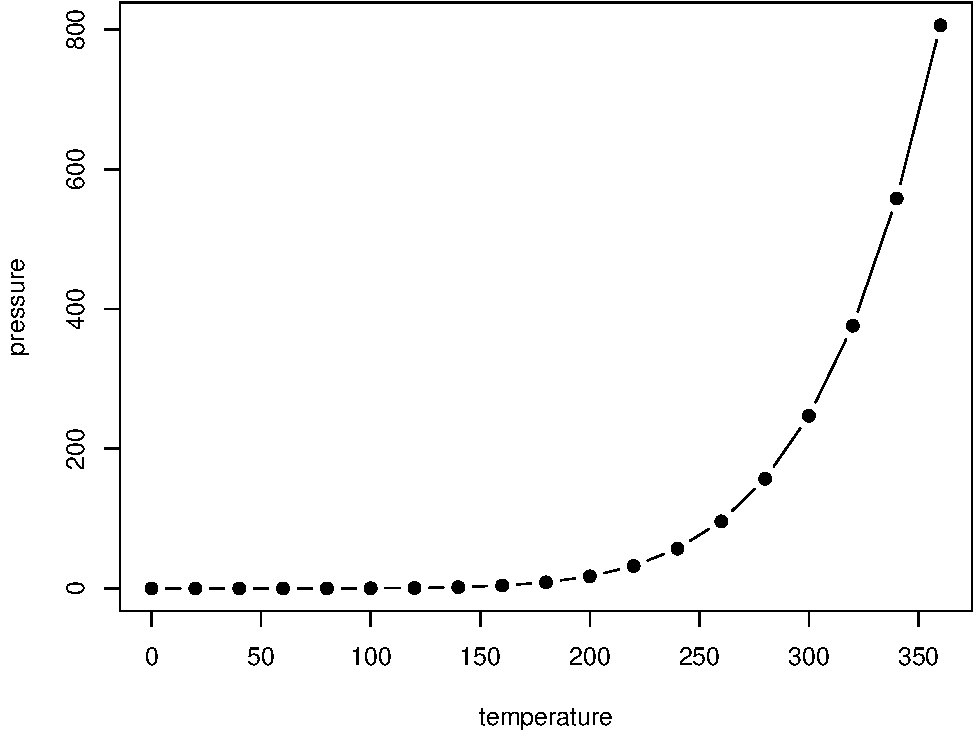
\includegraphics[width=0.8\linewidth]{_main_files/figure-latex/nice-fig-1} 

}

\caption{Here is a nice figure!}\label{fig:nice-fig}
\end{figure}

Don't miss Table \ref{tab:nice-tab}.

\begin{Shaded}
\begin{Highlighting}[]
\NormalTok{knitr}\SpecialCharTok{::}\FunctionTok{kable}\NormalTok{(}
  \FunctionTok{head}\NormalTok{(pressure, }\DecValTok{10}\NormalTok{), }\AttributeTok{caption =} \StringTok{\textquotesingle{}Here is a nice table!\textquotesingle{}}\NormalTok{,}
  \AttributeTok{booktabs =} \ConstantTok{TRUE}
\NormalTok{)}
\end{Highlighting}
\end{Shaded}

\begin{table}

\caption{\label{tab:nice-tab}Here is a nice table!}
\centering
\begin{tabular}[t]{rr}
\toprule
temperature & pressure\\
\midrule
0 & 0.0002\\
20 & 0.0012\\
40 & 0.0060\\
60 & 0.0300\\
80 & 0.0900\\
\addlinespace
100 & 0.2700\\
120 & 0.7500\\
140 & 1.8500\\
160 & 4.2000\\
180 & 8.8000\\
\bottomrule
\end{tabular}
\end{table}

\hypertarget{methodology}{%
\chapter{Methodology}\label{methodology}}

\hypertarget{variables}{%
\subsection{Variables}\label{variables}}

\hypertarget{categories-that-would-be-useful-things-to-predict}{%
\subsubsection{Categories that would be useful (things to predict?)}\label{categories-that-would-be-useful-things-to-predict}}

Owner-occupied?
Investor-owned?
Vacant?
Demolition in the past year (no construction since)
Construction in the past year

\hypertarget{factor-analysis-variables}{%
\subsubsection{factor analysis Variables}\label{factor-analysis-variables}}

The variables made it into the initial factor analysis were:

\begin{itemize}
\item
  Accessibility

  \begin{itemize}
  \tightlist
  \item
    Distance to transit (use number of transit stops within 1/2 mile walkshed)
  \item
    Share of old/new homes (use average age of homes within 1/2 mile walkshed)
  \item
    Transit frequency (use transit stops per hour within 1/2 mile walkshed)
  \end{itemize}
\item
  Affordability

  \begin{itemize}
  \tightlist
  \item
    Average Condition of homes in half-mile walkshed
  \item
    Median rent of block-groups with centroids within 1/2 mile walkshed.
  \item
    Median income of block groups with centroids within 1/2 mile walkshed.
  \item
    Median ownership cost of block groups with centroids within 1/2 mile walkshed.
  \end{itemize}
\item
  Close

  \begin{itemize}
  \tightlist
  \item
  \end{itemize}
\item
  Diverse buildings

  \begin{itemize}
  \tightlist
  \item
    Entropy of housing types (apartment, townhomes, etc) within 1/2 mile walkshed
  \end{itemize}
\item
  Other

  \begin{itemize}
  \tightlist
  \item
    Standard deviation of building age within 1/2 mile walkshed
  \end{itemize}
\end{itemize}

\hypertarget{data}{%
\section{Data}\label{data}}

We obtained data on property addresses, land uses, assessed values (for both
land and buildings), and building condition from the property assessment data
\citep{allegheny_county_office_of_property_assessments_allegheny_2022}, which
includes information on 582,116 properties in Allegheny County.

We also obtained latitude and longitude coordinates for each property from a
geocoder file provided by \citet{western_pennsylvania_regional_data_center_geocoders_2021}.
Over 99.5 percent of properties included in the assessment dataset are included
in the geocoder file. Properties without geocoded locations are excluded from
our analysis, leaving a total of 579,473 properties.

Potential development sites were identified as those

\begin{enumerate}
\def\labelenumi{\arabic{enumi}.}
\tightlist
\item
  classified as ``residential''
  (indicating residential properties with one to four housing units) or ``commercial''
  (which includes mixed-use developments and residential properties with more than four
  housing units) and
\item
  with a land use description in one of 59 possible categories. The most common of
  these are listed Table \ref{tab:list-site-uses}\footnote{The land use descriptions that were
    classified as potential development sites but are not listed in Table
    \ref{tab:list-site-uses}, which combine to represent less than one percent of all sites
    are ``RIGHTOF WAY - RESIDENTIAL'', ``CONDOMINIUM UNIT'', ``DWG USED AS OFFICE'', ``APART:20-39
    UNITS'', ``CONDO GARAGE UNITS'', ``COMMON AREA'', ``CONDO DEVELOPMENTAL LAND'',
    ``CONDEMNED/BOARDED-UP'', ``CONDOMINIUM OFFICE BUILDING'', ``INDEPENDENT LIVING (SENIORS)'',
    ``DWG USED AS RETAIL'', ``OTHER COMMERCIAL'', ``MOBILE HOMES/TRAILER PKS'', ``RIGHT OF WAY -
    COMMERCIAL'', ``GROUP HOME'', ``TOTAL/MAJOR FIRE DAMAGE - COMM'', ``OTHER COMMERCIAL HOUSING'',
    ``TOTAL/MAJOR FIRE DAMAGE'', ``COMM APRTM CONDOS 5-19 UNITS'', ``MUNICIPAL URBAN RENEWAL'',
    ``COMMERCIAL LAND'', ``CAMPGROUNDS'', ``COMMON AREA OR GREENBELT'', ``CHARITABLE
    EXEMPTION/HOS/HOMES'', ``INCOME PRODUCING PARKING LOT'', ``DWG APT CONVERSION'', ``\textgreater10 ACRES
    VACANT'', ``MINOR FIRE DAMAGE'', ``COMM APRTM CONDOS 20-39 UNITS'', ``COMMERCIAL/UTILITY'',
    ``H.O.A RECREATIONS AREA'', ``COMM APRTM CONDOS 40+ UNITS'', ``MINOR FIRE DAMAGE - COMM'',
    ``OTHER'', ``OTHER RESIDENTIAL STRUCTURE'', ``OWNED BY METRO HOUSING AU'', ``RESIDENTIAL VACANT
    LAND'', ``HUD PROJ \#221'', and ``VACANT LAND 0-9 ACRES''}. One site (3008 Phillip Dr in Clairton) is missing a land use description in the assessment data. We checked this address on Zillow to determine that this is a single-family home and classified it as such in our data.
\end{enumerate}

\begin{table}

\caption{\label{tab:list-site-uses}Most common land uses categorized as potential sites}
\centering
\begin{tabular}[t]{lrrr}
\toprule
USEDESC & Number of potential sites & Percent of potential sites & Cumulative percent of potential sites\\
\midrule
SINGLE FAMILY & 371,064 & 69.8 & 69.8\\
VACANT LAND & 63,603 & 12.0 & 81.7\\
TWO FAMILY & 17,330 & 3.3 & 85.0\\
CONDOMINIUM & 16,683 & 3.1 & 88.1\\
TOWNHOUSE & 14,953 & 2.8 & 90.9\\
\addlinespace
ROWHOUSE & 11,129 & 2.1 & 93.0\\
VACANT COMMERCIAL LAND & 6,103 & 1.1 & 94.2\\
THREE FAMILY & 3,977 & 0.7 & 94.9\\
RES AUX BUILDING (NO HOUSE) & 3,635 & 0.7 & 95.6\\
RETL/APT'S OVER & 3,366 & 0.6 & 96.2\\
\addlinespace
COMM AUX BUILDING & 3,040 & 0.6 & 96.8\\
APART: 5-19 UNITS & 2,800 & 0.5 & 97.3\\
MOBILE HOME (IN PARK) & 2,563 & 0.5 & 97.8\\
FOUR FAMILY & 2,064 & 0.4 & 98.2\\
BUILDERS LOT & 1,714 & 0.3 & 98.5\\
\addlinespace
CONDOMINIUM COMMON PROPERTY & 1,307 & 0.2 & 98.8\\
PARKING GARAGE/LOTS & 935 & 0.2 & 99.0\\
OFFICE/APARTMENTS OVER & 860 & 0.2 & 99.1\\
MOBILE HOME & 676 & 0.1 & 99.2\\
APART:40+ UNITS & 545 & 0.1 & 99.3\\
\bottomrule
\end{tabular}
\end{table}

The above criteria yield 531,811 potential sites. Potential building sites were
further filtered to exclude those with missing data on the most recent sale
(6,574 sites, or about one percent of all sites).\footnote{Four sites had sales prices
  listed that were unreasonably high. 3039 Liberty Avenue in Pittsburgh is listed
  as having sold for \$511,945,000 on August 30, 2021. Zillow lists this property
  as having sold on that date for \$511,945
  (\url{https://www.zillow.com/homedetails/3039-W-Liberty-Ave-Pittsburgh-PA-15216/2070262638_zpid/}, accessed 5/4/2022),
  so the value was corrected for what appears to have been a typo. 220 Hyeholde Dr
  in Coraopolis is listed as having sold for \$28,100,000 in 1967. This may also
  be a typo, and it also does not seem to be the most recent sale. Zillow lists
  this home as having sold for \$350,000 in 2004
  (\url{https://www.zillow.com/homes/220-hyeholde-dr,-Coraopolis,-PA_rb/11552817_zpid/},
  accessed 5/4/2022), so the data was corrected to add that as the most recent sale.
  Two other sites were identified as having unreasonably high sales values: 1339
  Arlington Avenue in Pittsburgh is a three-bedroom single-family home that is
  listed as having sold for \$57,010,813 in 1976 and a 0.06-acre vacant lot with
  tax ID 0165G00270000000 is listed as having sold for \$24,920,232 in 1936. The
  sales data for these sites were treated as missing.} for a total of 526,237
potential sites.

The focus of this analysis is on potential development sites rather than on
properties. Some properties in the assessor dataset are condominums where
multiple properties share a single parcel of land. We aggregated these to the
site level by identifying all properties with an assessed building value
greater than zero, a land value of zero, and a land use description that did
not indicate the land was vacant. If multiple such properties share an address,
we classified all properties at that address as a condominium and aggregated
them to the parcel level. This led to a final sample of 518,316 sites.

\hypertarget{aspatial-data}{%
\subsection{Aspatial data}\label{aspatial-data}}

Three variables (total assessed fair market value, assessed fair market value of the building, and lot area) were taken directly from the assessment data for use in our analysis. We calculated two additional variables from the assessment data: the inflation-adjusted sales price and the average number of years between sales. The average of:

\begin{enumerate}
\def\labelenumi{\arabic{enumi}.}
\tightlist
\item
  The number of years between the most recent sale and the publication data of the assessment data (May 1, 2022);
\item
  The number of years between the most recent sale and the second-most recent sale\footnote{If no date is listed for the second-most recent sale, we used January 1, 1950. The data user guide notes that, although deeds have been recorded in Allegheny County since 1788 (and the earliest sale listed in the data is from November 24, 1806), early sales may not be included in the electronic system and may default to a 1950 sale date \citep{western_pennsylvania_regional_data_center_allegheny_2017}. This effects about one third of parcels in our dataset.}; and
\item
  The number of years between the second-most recent sale and the third-most recent sale, if a third-most recent sale is listed.
\end{enumerate}

To aggregate properties identified as condominiums to the site level, we summed
the total values for lot area, assessed land value, assessed building value, and
inflation-adjusted sale price and averaged values for the average number of
years between sales.

\begin{Shaded}
\begin{Highlighting}[]
\FunctionTok{write\_csv}\NormalTok{(sites,}
          \FunctionTok{here}\NormalTok{(}\StringTok{"data"}\NormalTok{,}
               \StringTok{"sites.csv"}\NormalTok{))}
\end{Highlighting}
\end{Shaded}

\hypertarget{accessibilty-data}{%
\subsection{Accessibilty data}\label{accessibilty-data}}

Accessibilty was calculated from each of the 518,316 sites in our sample to
each of several location types described below.

We used land use codes from the county assessor parcel data to identify
\emph{destination parcels} that residents might value access to. The most common
land use codes of identified destination parcels are listed in \ref{tab:dest-uses}.

\begin{table}

\caption{\label{tab:dest-uses}Land uses identified as potential destinations}
\centering
\begin{tabular}[t]{lrrr}
\toprule
USEDESC & Number of identified destinations & Percent of identified destinations & Cumulative percent of identified destinations\\
\midrule
MUNICIPAL GOVERNMENT & 10,378 & 29.88 & 29.88\\
CHURCHES, PUBLIC WORSHIP & 1,948 & 5.61 & 35.49\\
COMMERCIAL GARAGE & 1,735 & 5.00 & 40.49\\
OFFICE - 1-2 STORIES & 1,649 & 4.75 & 45.23\\
SMALL DETACHED RET(UNDER 10000) & 1,645 & 4.74 & 49.97\\
\addlinespace
OFFICE/WAREHOUSE & 1,385 & 3.99 & 53.96\\
COUNTY GOVERNMENT & 1,287 & 3.71 & 57.66\\
WAREHOUSE & 1,255 & 3.61 & 61.28\\
OWNED BY BOARD OF EDUCATION & 1,086 & 3.13 & 64.41\\
TOWNSHIP GOVERNMENT & 853 & 2.46 & 66.86\\
\addlinespace
LIVESTOCK O/T D \& P-CAUV & 805 & 2.32 & 69.18\\
LIGHT MANUFACTURING & 799 & 2.30 & 71.48\\
PUBLIC PARK & 710 & 2.04 & 73.52\\
RESTAURANT, CAFET AND/OR BAR & 697 & 2.01 & 75.53\\
GENERAL FARM & 607 & 1.75 & 77.28\\
\addlinespace
OWNED BY COLLEGE/UNIV/ACADEMY & 458 & 1.32 & 78.60\\
MEDICAL CLINICS/OFFICES & 445 & 1.28 & 79.88\\
RETL/OFF OVER & 442 & 1.27 & 81.15\\
OFFICE-ELEVATOR -3 + STORIES & 413 & 1.19 & 82.34\\
LODGE HALL/AMUSEMENT PARK & 386 & 1.11 & 83.45\\
\addlinespace
AUTO SALES \& SERVICE & 364 & 1.05 & 84.50\\
RETL/STOR OVER & 344 & 0.99 & 85.49\\
CEMETERY/MONUMENTS & 340 & 0.98 & 86.47\\
STATE GOVERNMENT & 331 & 0.95 & 87.42\\
CONVENIENCE STORE/GAS & 304 & 0.88 & 88.30\\
\addlinespace
BANK & 298 & 0.86 & 89.16\\
NEIGH SHOP CENTER & 297 & 0.86 & 90.01\\
BARS & 240 & 0.69 & 90.70\\
FUNERAL HOMES & 194 & 0.56 & 91.26\\
DAYCARE/PRIVATE SCHOOL & 191 & 0.55 & 91.81\\
\addlinespace
MINI WAREHOUSE & 182 & 0.52 & 92.34\\
MEDIUM MANUFACTURING & 172 & 0.50 & 92.83\\
NURSING HOME/PRIVATE HOS & 171 & 0.49 & 93.32\\
DRIVE IN REST OR FOOD SERVICE & 170 & 0.49 & 93.81\\
OFFICE-WALKUP -3 + STORIES & 164 & 0.47 & 94.28\\
\addlinespace
AUTO SERV STATION & 137 & 0.39 & 94.68\\
COMMUNITY SHOPPING CENTER & 137 & 0.39 & 95.07\\
OTHER RETAIL STRUCTURES & 135 & 0.39 & 95.46\\
WAREHOUSE/MULTI-TENANT & 126 & 0.36 & 95.82\\
BOWLING ALLEYS/REC FACILITY & 120 & 0.35 & 96.17\\
\addlinespace
HOTELS & 113 & 0.33 & 96.50\\
DISCOUNT STORE & 110 & 0.32 & 96.81\\
CAR WASH & 103 & 0.30 & 97.11\\
FAST FOOD/DRIVE THRU WINDOW & 85 & 0.24 & 97.35\\
PHARMACY (CHAIN) & 85 & 0.24 & 97.60\\
\addlinespace
SMALL SHOP & 81 & 0.23 & 97.83\\
SUPERMARKETS & 75 & 0.22 & 98.05\\
OFFICE/STORAGE OVER & 66 & 0.19 & 98.24\\
COUNTRY CLUBS & 55 & 0.16 & 98.40\\
REGIONAL SHOPPING CENTER & 50 & 0.14 & 98.54\\
\addlinespace
OFFICE/RETAIL OVER & 46 & 0.13 & 98.67\\
DRY CLEANING PLANTS/LAUNDRIES & 44 & 0.13 & 98.80\\
MOTEL \& TOURIST CABINS & 42 & 0.12 & 98.92\\
BIG BOX RETAIL & 38 & 0.11 & 99.03\\
CONVENIENCE STORE & 36 & 0.10 & 99.13\\
\addlinespace
LIVE STOCK FARM & 34 & 0.10 & 99.23\\
MARINA & 34 & 0.10 & 99.33\\
DEPARTMENT STORE & 32 & 0.09 & 99.42\\
GREENHOUSES, VEG \& FLORACULTURE & 29 & 0.08 & 99.50\\
THEATER & 29 & 0.08 & 99.59\\
\addlinespace
GOLF DRIVING RANGE/MINIATURE & 22 & 0.06 & 99.65\\
GOLF COURSES (PUBLIC) & 20 & 0.06 & 99.71\\
BED \& BREAKFAST & 15 & 0.04 & 99.75\\
OTHER AGRICULTURAL - CAUV & 14 & 0.04 & 99.79\\
SAVINGS AND LOANS & 12 & 0.03 & 99.83\\
\addlinespace
OTHER FOOD SERVICE & 11 & 0.03 & 99.86\\
NURSERY & 9 & 0.03 & 99.88\\
CASINO & 7 & 0.02 & 99.90\\
CONVENIENCE STORE GAS/REPAIRS & 7 & 0.02 & 99.93\\
MARINE SERV FACILITY & 7 & 0.02 & 99.95\\
\addlinespace
FORESTRY WITH BUILDING & 5 & 0.01 & 99.96\\
HEAVY EQUIPMENT SALES/RENTAL & 5 & 0.01 & 99.97\\
GAS STATION KIOSK & 3 & 0.01 & 99.98\\
VEGETABLE FARM & 3 & 0.01 & 99.99\\
TIMBER OR FOREST LAND & 2 & 0.01 & 100.00\\
\addlinespace
FORESTRY W/BUILDINGS & 1 & 0.00 & 100.00\\
\bottomrule
\end{tabular}
\end{table}

We identified \emph{job locations} based on data from a Longitudinal
Employer-Household Dynamics (LEHD) dataset published by the United States Census
Bureau \citep{united_states_census_bureau_lehd_2021}. The LEHD dataset provides the
total number of jobs in each census block in the United States, based on
employment tax records. The location of each job was defined as the centroid of
the block in which it was located. We downloaded job location data for
Pennsylvania and filtered it to include locations in the Pittsburgh metropolitan
area (Allegheny, Armstrong, Beaver, Butler, Fayette, Washington, and
Westmoreland counties).

In addition to calculating the accessibility to jobs of all categories, we also
calculated accessibility to several subsets of jobs. We disaggregated jobs by
earnings, reasoning that the usefulness of a job might vary depending on how
well it matches a workers skills or wage expectations. \emph{High-paying job locations}
are a subset of job locations where the worker earns more than \$3333 per month.
\emph{Low-paying job locations} are those where the worker earns \$1250 per month or less.

We also disaggregated jobs based on employment industry, based on the North
American Industry Classification System (NAICS), reasoning that the presence of
jobs particular industries might represent a shopping or recreation destination.
\emph{Retail job locations} are a subset of job locations in NAICS sector 44-45
(retail trade); \emph{Entertainment job locations} are those in NAICS sector 71
(arts, entertainment, and recreation); and \emph{Hospitality job locations} are
those in NAICS sector 72 (accommodation and food services).

Finally we identified three location types that correspond with common non-work
trips: schools, grocery stores, and parks. \emph{Grocery store locations} were
identified as vendors participating in the Supplemental Nutrition Program for
Women, Infants, and Children (WIC). WIC vendor locations and \emph{school locations}
were obtained from the and location data came from the Allegheny County GIS portal
\citep{allegheny_county_office_of_information_technology_allegheny_2018, allegheny_county_office_of_information_technology_allegheny_2020}.
\emph{Park locations} were taken from the Pennsylvania Geospatial Data Clearinghouse
\citep{pennsylvania_department_of_conservation_and_natural_resources_pennsylvania_2015}.
Data were downloaded for Pennsylvania and filtered to Allegheny county.

We used the r5r package in the R programming language \citep{pereira_r5r_2021} to
calculate accessibility was calculated for each destination type described above
for each of four transportation modes (walking, cycling, driving, and transit).
The r5r package calculates accessibility as the weighted total number of
destinations reachable by a given mode, where destinations are weighted
according to a decay function, such that destinations that can be reached within
less time are assigned greater weight. We used a logistic decay function, as
illustrated in \ref{fig:show-decay-func}. For motorized modes, the decay
function had a mean (inflection) of 40 minutes and a standard deviation of 10
minutes. For non-motorized modes, the decay function had a mean of 20 minutes
and a standard deviation of 5 minutes.

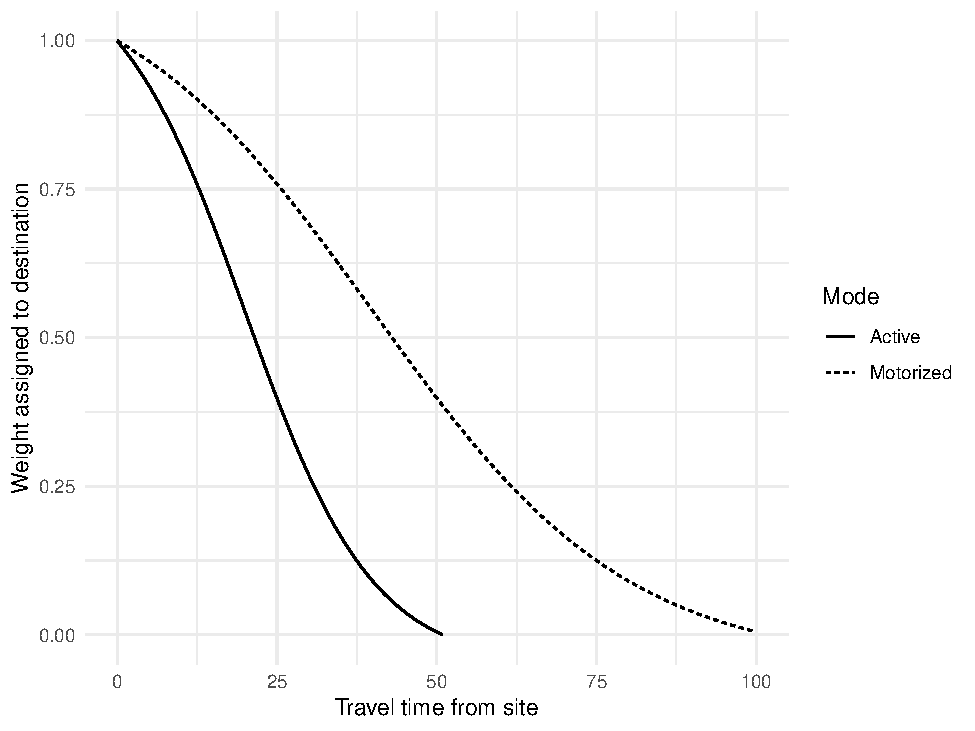
\includegraphics{_main_files/figure-latex/show-decay-func-1.pdf}

Calculating accessibility metrics for a combination of four transportation modes
and ten destination types yeilds 40 different accessibility variables.

\hypertarget{density-data}{%
\subsection{Density data}\label{density-data}}

For each site, we calculated the density of four different (dis)amenites in the
immediates vicinity (defined as the area within a one-kilometer radius): homes,
pedestrian paths (including sidewalks and all routes open to pedestrians), roads
that are not open to pedestrians (such as freeways), and land uses identified
in county assessor data as one of several types that we categorized as
disamenities. The land use codes we used to identify disamenities are listed in

\begin{itemize}
\tightlist
\item
  Housing density (use number of homes within 1/2 mile circle)
\item
  Ped network density (use mileage of ped network within 1/2 mile circle)
\item
  Number of disamenities in a 1/2 mile circle
\item
  Mileage of non-ped roads in 1/2 mile circle
\end{itemize}

\hypertarget{footnotes-and-citations}{%
\chapter{Footnotes and citations}\label{footnotes-and-citations}}

\hypertarget{footnotes}{%
\section{Footnotes}\label{footnotes}}

Footnotes are put inside the square brackets after a caret \texttt{\^{}{[}{]}}. Like this one \footnote{This is a footnote.}.

\hypertarget{citations}{%
\section{Citations}\label{citations}}

Reference items in your bibliography file(s) using \texttt{@key}.

For example, we are using the \textbf{bookdown} package \citep{R-bookdown} (check out the last code chunk in index.Rmd to see how this citation key was added) in this sample book, which was built on top of R Markdown and \textbf{knitr} \citep{xie2015} (this citation was added manually in an external file book.bib).
Note that the \texttt{.bib} files need to be listed in the index.Rmd with the YAML \texttt{bibliography} key.

The RStudio Visual Markdown Editor can also make it easier to insert citations: \url{https://rstudio.github.io/visual-markdown-editing/\#/citations}

\hypertarget{blocks}{%
\chapter{Blocks}\label{blocks}}

\hypertarget{equations}{%
\section{Equations}\label{equations}}

Here is an equation.

\begin{equation} 
  f\left(k\right) = \binom{n}{k} p^k\left(1-p\right)^{n-k}
  \label{eq:binom}
\end{equation}

You may refer to using \texttt{\textbackslash{}@ref(eq:binom)}, like see Equation \eqref{eq:binom}.

\hypertarget{theorems-and-proofs}{%
\section{Theorems and proofs}\label{theorems-and-proofs}}

Labeled theorems can be referenced in text using \texttt{\textbackslash{}@ref(thm:tri)}, for example, check out this smart theorem \ref{thm:tri}.

\begin{theorem}
\protect\hypertarget{thm:tri}{}\label{thm:tri}For a right triangle, if \(c\) denotes the \emph{length} of the hypotenuse
and \(a\) and \(b\) denote the lengths of the \textbf{other} two sides, we have
\[a^2 + b^2 = c^2\]
\end{theorem}

Read more here \url{https://bookdown.org/yihui/bookdown/markdown-extensions-by-bookdown.html}.

\hypertarget{callout-blocks}{%
\section{Callout blocks}\label{callout-blocks}}

The R Markdown Cookbook provides more help on how to use custom blocks to design your own callouts: \url{https://bookdown.org/yihui/rmarkdown-cookbook/custom-blocks.html}

\hypertarget{sharing-your-book}{%
\chapter{Sharing your book}\label{sharing-your-book}}

\hypertarget{publishing}{%
\section{Publishing}\label{publishing}}

HTML books can be published online, see: \url{https://bookdown.org/yihui/bookdown/publishing.html}

\hypertarget{pages}{%
\section{404 pages}\label{pages}}

By default, users will be directed to a 404 page if they try to access a webpage that cannot be found. If you'd like to customize your 404 page instead of using the default, you may add either a \texttt{\_404.Rmd} or \texttt{\_404.md} file to your project root and use code and/or Markdown syntax.

\hypertarget{metadata-for-sharing}{%
\section{Metadata for sharing}\label{metadata-for-sharing}}

Bookdown HTML books will provide HTML metadata for social sharing on platforms like Twitter, Facebook, and LinkedIn, using information you provide in the \texttt{index.Rmd} YAML. To setup, set the \texttt{url} for your book and the path to your \texttt{cover-image} file. Your book's \texttt{title} and \texttt{description} are also used.

This \texttt{gitbook} uses the same social sharing data across all chapters in your book- all links shared will look the same.

Specify your book's source repository on GitHub using the \texttt{edit} key under the configuration options in the \texttt{\_output.yml} file, which allows users to suggest an edit by linking to a chapter's source file.

Read more about the features of this output format here:

\url{https://pkgs.rstudio.com/bookdown/reference/gitbook.html}

Or use:

\begin{Shaded}
\begin{Highlighting}[]
\NormalTok{?bookdown}\SpecialCharTok{::}\NormalTok{gitbook}
\end{Highlighting}
\end{Shaded}


  \bibliography{book.bib,packages.bib}

\end{document}
